\documentclass[journal,12pt,twocolumn]{IEEEtran}

\usepackage{setspace}
\usepackage{gensymb}
\singlespacing
\usepackage[cmex10]{amsmath}

\usepackage{amsthm}

\usepackage{mathrsfs}
\usepackage{txfonts}
\usepackage{stfloats}
\usepackage{bm}
\usepackage{cite}
\usepackage{cases}
\usepackage{subfig}

\usepackage{longtable}
\usepackage{multirow}

\usepackage{enumitem}
\usepackage{mathtools}
\usepackage{steinmetz}
\usepackage{tikz}
\usepackage{circuitikz}
\usepackage{verbatim}
\usepackage{tfrupee}
\usepackage[breaklinks=true]{hyperref}
\usepackage{graphicx}
\usepackage{tkz-euclide}

\usetikzlibrary{calc,math}
\usepackage{listings}
    \usepackage{color}                                            %%
    \usepackage{array}                                            %%
    \usepackage{longtable}                                        %%
    \usepackage{calc}                                             %%
    \usepackage{multirow}                                         %%
    \usepackage{hhline}                                           %%
    \usepackage{ifthen}                                           %%
    \usepackage{lscape}     
\documentclass[journal,12pt,twocolumn]{IEEEtran}

\usepackage{setspace}
\usepackage{gensymb}
\singlespacing
\usepackage[cmex10]{amsmath}

\usepackage{amsthm}

\usepackage{mathrsfs}
\usepackage{txfonts}
\usepackage{stfloats}
\usepackage{bm}
\usepackage{cite}
\usepackage{cases}
\usepackage{subfig}

\usepackage{longtable}
\usepackage{multirow}

\usepackage{enumitem}
\usepackage{mathtools}
\usepackage{steinmetz}
\usepackage{tikz}
\usepackage{circuitikz}
\usepackage{verbatim}
\usepackage{tfrupee}
\usepackage[breaklinks=true]{hyperref}
\usepackage{graphicx}
\usepackage{tkz-euclide}

\usetikzlibrary{calc,math}
\usepackage{listings}
    \usepackage{color}                                            %%
    \usepackage{array}                                            %%
    \usepackage{longtable}                                        %%
    \usepackage{calc}                                             %%
    \usepackage{multirow}                                         %%
    \usepackage{hhline}                                           %%
    \usepackage{ifthen}                                           %%
    \usepackage{lscape}     
\usepackage{multicol}
\usepackage{chngcntr}

\DeclareMathOperator*{\Res}{Res}

\renewcommand\thesection{\arabic{section}}
\renewcommand\thesubsection{\thesection.\arabic{subsection}}
\renewcommand\thesubsubsection{\thesubsection.\arabic{subsubsection}}

\renewcommand\thesectiondis{\arabic{section}}
\renewcommand\thesubsectiondis{\thesectiondis.\arabic{subsection}}
\renewcommand\thesubsubsectiondis{\thesubsectiondis.\arabic{subsubsection}}


\hyphenation{op-tical net-works semi-conduc-tor}
\def\inputGnumericTable{}                                 %%

\lstset{
%language=C,
frame=single, 
breaklines=true,
columns=fullflexible
}
\begin{document}


\newtheorem{theorem}{Theorem}[section]
\newtheorem{problem}{Problem}
\newtheorem{proposition}{Proposition}[section]
\newtheorem{lemma}{Lemma}[section]
\newtheorem{corollary}[theorem]{Corollary}
\newtheorem{example}{Example}[section]
\newtheorem{definition}[problem]{Definition}

\newcommand{\BEQA}{\begin{eqnarray}}
\newcommand{\EEQA}{\end{eqnarray}}
\newcommand{\define}{\stackrel{\triangle}{=}}
\bibliographystyle{IEEEtran}
\raggedbottom
\setlength{\parindent}{0pt}
\providecommand{\mbf}{\mathbf}
\providecommand{\pr}[1]{\ensuremath{\Pr\left(#1\right)}}
\providecommand{\qfunc}[1]{\ensuremath{Q\left(#1\right)}}
\providecommand{\sbrak}[1]{\ensuremath{{}\left[#1\right]}}
\providecommand{\lsbrak}[1]{\ensuremath{{}\left[#1\right.}}
\providecommand{\rsbrak}[1]{\ensuremath{{}\left.#1\right]}}
\providecommand{\brak}[1]{\ensuremath{\left(#1\right)}}
\providecommand{\lbrak}[1]{\ensuremath{\left(#1\right.}}
\providecommand{\rbrak}[1]{\ensuremath{\left.#1\right)}}
\providecommand{\cbrak}[1]{\ensuremath{\left\{#1\right\}}}
\providecommand{\lcbrak}[1]{\ensuremath{\left\{#1\right.}}
\providecommand{\rcbrak}[1]{\ensuremath{\left.#1\right\}}}
\theoremstyle{remark}
\newtheorem{rem}{Remark}
\newcommand{\sgn}{\mathop{\mathrm{sgn}}}
\providecommand{\abs}[1]{$\left\vert#1\right\vert$}
\providecommand{\res}[1]{\Res\displaylimits_{#1}} 
\providecommand{\norm}[1]{$\left\lVert#1\right\rVert$}
%\providecommand{\norm}[1]{\lVert#1\rVert}
\providecommand{\mtx}[1]{\mathbf{#1}}
\providecommand{\mean}[1]{E$\left[ #1 \right]$}
\providecommand{\fourier}{\overset{\mathcal{F}}{ \rightleftharpoons}}
%\providecommand{\hilbert}{\overset{\mathcal{H}}{ \rightleftharpoons}}
\providecommand{\system}{\overset{\mathcal{H}}{ \longleftrightarrow}}
	%\newcommand{\solution}[2]{\textbf{Solution:}{#1}}
\newcommand{\solution}{\noindent \textbf{Solution: }}
\newcommand{\cosec}{\,\text{cosec}\,}
\providecommand{\dec}[2]{\ensuremath{\overset{#1}{\underset{#2}{\gtrless}}}}
\newcommand{\myvec}[1]{\ensuremath{\begin{pmatrix}#1\end{pmatrix}}}
\newcommand{\mydet}[1]{\ensuremath{\begin{vmatrix}#1\end{vmatrix}}}
\numberwithin{equation}{subsection}
\makeatletter
\@addtoreset{figure}{problem}
\makeatother
\let\StandardTheFigure\thefigure
\let\vec\mathbf
\renewcommand{\thefigure}{\theproblem}
\def\putbox#1#2#3{\makebox[0in][l]{\makebox[#1][l]{}\raisebox{\baselineskip}[0in][0in]{\raisebox{#2}[0in][0in]{#3}}}}
     \def\rightbox#1{\makebox[0in][r]{#1}}
     \def\centbox#1{\makebox[0in]{#1}}
     \def\topbox#1{\raisebox{-\baselineskip}[0in][0in]{#1}}
     \def\midbox#1{\raisebox{-0.5\baselineskip}[0in][0in]{#1}}
\vspace{3cm}
\title{Assignment 1}
\author{Akyam L Dhatri Nanda - AI20BTECH11002}
\maketitle
\newpage
\bigskip
\renewcommand{\thefigure}{\theenumi}
\renewcommand{\thetable}{\theenumi}
Download all python codes from 
\begin{lstlisting}
https://github.com/Dhatri-nanda/EE3900/blob/main/Assignment_1/code.py
\end{lstlisting}
%
and latex-tikz codes from 
%
\begin{lstlisting}
https://github.com/Dhatri-nanda/EE3900/blob/main/Assignment_1/Assignment_1.tex
\end{lstlisting}
\section{Problem}
Prove that the points $\myvec{21\\-2}$, $\myvec{15\\10}$, $\myvec{-5\\0}$, $\myvec{1\\-12}$ are the vertices of a rectangle, and find the coordinates of its centre.

\section{Solution}
\begin{lemma}
In a quadrilateral ABCD, if opposite sides are parallel, then those opposite sides are equal
\end{lemma}
\begin{proof}
For $\triangle ABC and \triangle CDA$
\begin{align}
    \angle{BAC} &= \angle{DCA}\\
    \angle{BCA} &= \angle{DAC}\\
    AC &= CA
\end{align}
By AAS congruency, $\triangle ABC = \triangle CDA$

So, AB = CD and BC = AD
\end{proof}
\begin{lemma}
In a quadrilateral ABCD having equal and opposite parallel sides, any two adjacent or consecutive angles are supplementary.
 \label{lemma 2}
\end{lemma} 
\begin{proof}
AB $||$ CD and AD is transversal

We know that interior angles on the same side of a transversal are supplementary.

Therefore,
\begin{align}
    \angle A + \angle D = 180\degree
\end{align}
Similarly,
\begin{align}
    \angle B + \angle C = 180\\
    \angle C + \angle D = 180\\
    \angle A + \angle B = 180
\end{align}
\end{proof}
A rectangle is a quadrilateral with equal opposite sides(unequal adjacent sides) and all angles as right angles.

Let's name the points as A,B,C and D respectively i.e.,
\begin{align}
\vec{A} = \myvec{21\\-2}
\vec{B} = \myvec{15\\10}
\vec{C} = \myvec{-5\\0}
\vec{D} = \myvec{1\\-12}\label{eq 2.0.1}
\end{align}

The minimum verification is the opposite sides to be parallel and one angle is right angle with unequal adjacent sides.

So, first we check if opposite sides are parallel

Two lines are parallel if their respective
directional vectors are in the same ratio

The directional vector of $\vec{AB}$ is
\begin{align}
    = \myvec{21-15 \\ -2-10} = \myvec{6 \\ -12}
\end{align}

The directional vector of $\vec{BC}$ is
\begin{align}
    = \myvec{15+5 \\ 10-0} = \myvec{20 \\ 10}
\end{align}

The directional vector of $\vec{CD}$ is
\begin{align}
    = \myvec{-5-1 \\ 0+12} = \myvec{-6 \\ 12}
\end{align}

The directional vector of $\vec{DA}$ is
\begin{align}
    = \myvec{-21+1 \\ 2-12} = \myvec{-20 \\ -10}
\end{align}

Since the directional vectors of $\vec{AB}$ and $\vec{CD}$
are in the same ratio, so  $\vec{AB}$ and $\vec{CD}$ are
parallel and also opposite to each other.
Similarly, $\vec{BC}$ and $\vec{DA}$ are parallel and opposite.

So, from lemma \ref{lemma 2} opposite sides are equal.
Next, we find one of the angle
\begin{align}
    \angle B &= (\vec{\vec{B} - \vec{A}})^\top(\vec{\vec{C} - \vec{B}}) \\ 
    &= \myvec{-6 & 12} \myvec{-20 \\ -10}\\
    &= 0
\end{align}
Therefore, one of the angle is right angle.

And from lemma \ref{lemma 2}, we can say all angles are right angles.

Next, 
\begin{align}
    \norm{\vec{A} - \vec{B}} = \sqrt{6^2 + 12^2} = \sqrt{180}\\
    \norm{\vec{B} - \vec{C}} = \sqrt{20^2 + 12^2} = \sqrt{544}
\end{align}
So, adjacent sides are not equal.

Therefore, we have proved that the above conditions are sufficient for defining a rectangle like we have defined above.
So, the given vertices form a rectangle.

The center($\vec{O}$) of any quadrilateral is the midpoint of it's diagonal. 
\begin{align}
    \vec{O} &= \frac{\vec{A}+ \vec{C}}{2}\\
    &= \myvec{8 \\ -1}
\end{align}

\begin{figure}[htp]
    \centering
    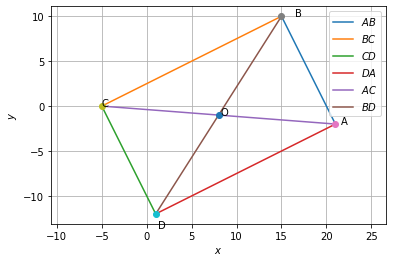
\includegraphics[width=\columnwidth]{AS1.png}
    \caption{plot}
    \label{fig:my_label}
\end{figure}
\end{document}
